\documentclass[11pt, oneside]{article}   	% use "amsart" instead of "article" for AMSLaTeX format
\usepackage{geometry}                		% See geometry.pdf to learn the layout options. There are lots.
\geometry{letterpaper}                   		% ... or a4paper or a5paper or ... 
%\geometry{landscape}                		% Activate for for rotated page geometry
%\usepackage[parfill]{parskip}    		% Activate to begin paragraphs with an empty line rather than an indent
\usepackage{graphicx}				% Use pdf, png, jpg, or eps� with pdflatex; use eps in DVI mode
								% TeX will automatically convert eps --> pdf in pdflatex		
\usepackage{amssymb}
\usepackage{amsmath}

\title{Center of Mass}
%\author{The Author}
%\section{}
% \subsection*{R code}
\date{}							% Activate to display a given date or no date

\graphicspath{{/Users/telliott_admin/Dropbox/Tex/png/}}

% \begin{center} 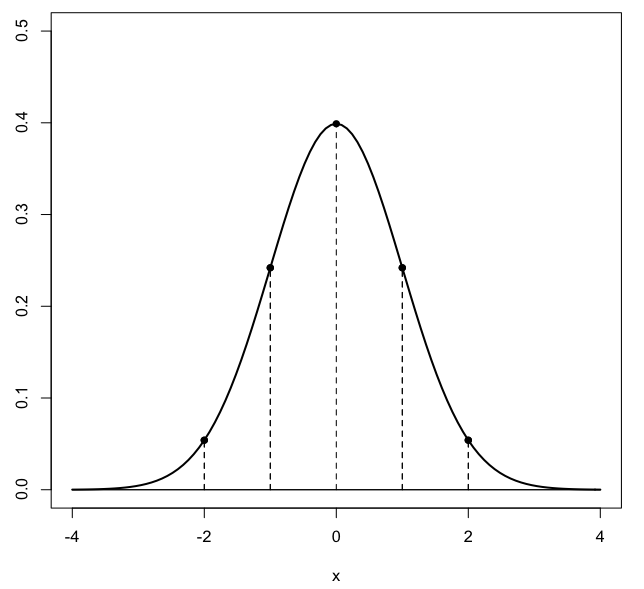
\includegraphics [scale=0.4] {gauss3.png} \end{center}
% \begin{bmatrix} a  &  b \\ c  &  d \end{bmatrix}
% \bigg |_

\begin{document}
\maketitle
\large
%\noindent

As you know, in single variable calculus we can interpret
\[ \int_a^b f(x) dx \]
as the area underneath the curve $y=f(x)$ between the lines $x=a$ and $x=b$ (our limits).  In multi-variable calculus we compute the double integral over the same region as follows
\[ \int_{x=a}^{x=b} \int_{y=0}^{y=f(x)} dy \ dx =  \int_{x=a}^b y \bigg |_0^{f(x)}  \ dx = \int_a^b f(x) \ dx \]
To be more general, we'd just say that we compute the double integral over the region $R$
\[ \iint\limits_{R} dx \ dy  \]
with the understanding that we can compute the inner integral with respect to either $x$ or $y$, whichever is more convenient.
Another difference from the single-variable approach is that we can extend this approach by computing
\[ \iint\limits_{R} g(x,y) \ dx \ dy  \]
Suppose, for example, that $g(x,y)$ is a function that gives the density of a flat object for each coordinate $x,y$.  In this case we usually use the label $\rho (x,y)$.  This integral gives the total mass of the object:
\[ M = \iint\limits_{R} \rho (x,y) \ dx \ dy  \]
To find the center of mass we compute
\[ M_x = \iint\limits_{R} \rho (x,y)\  y \ dx \ dy  \]
\[ M_y = \iint\limits_{R} \rho (x,y) \ x \ dx \ dy \]
And then finally 
\[ \bar{x} = \frac{M_x}{M} \]
\[ \bar{y} = \frac{M_y}{M} \]
\vspace{5 mm}

\noindent
Let's do a simple example.  Suppose our region is a rectangle with the origin as one corner and the point $(1,2)$ as the opposite corner.  It's just a 2D box of width $1$ and height $2$.  And let's say our density function is $\rho (x,y) = xy$.  Then
\[ M = \iint\limits_{R} \rho (x,y) \ dx \ dy =  \int_{y=0}^{y=2} \int_{x=0}^{x=1} xy \ dx \ dy  \]
The inner integral is
\[ \frac{1}{2} x^2 y \ \bigg |_0^{1} = \frac{1}{2} y \]
and the rest is
\[ M = \int_{y=0}^{y=2} \frac{1}{2} y \ dy = \frac{1}{4} y^2 \  \bigg |_0^{2} = 1 \]
Now
\[ M_x =  \int_{y=0}^{y=2} \int_{x=0}^{x=1} xy^2 \ dx \ dy  \]
The inner integral is
\[ \frac{1}{2} x^2 y^2 \ \bigg |_0^{1} = \frac{1}{2} y^2 \]
and the rest is
\[ M_x  = \int_{y=0}^{y=2} \frac{1}{2} y^2 \ dy = \frac{1}{6} y^3 \  \bigg |_0^{2} = \frac{4}{3} \]
Last, $M_y$ can be done in the same order
\[ M_y =  \int_{y=0}^{y=2} \int_{x=0}^{x=1} x^2y \ dx \ dy  \]
The inner integral is
\[ \frac{1}{3} x^3 y \ \bigg |_0^{1} = \frac{1}{3} y \]
and the rest is
\[ M_y  = \int_{y=0}^{y=2} \frac{1}{3} y \ dy = \frac{1}{6} y^2 \  \bigg |_0^{2} = \frac{2}{3} \]
Thus our center of mass is at the point $2/3,4/3$.  If it had made our lives easier, either integral could be computed with respect to $y$ before $x$.
The answer makes sense.  The density increases as we go to the right and up, so the center of mass is offset from the geometric center in the same direction.


\end{document}  